\documentclass[10pt]{article}
\usepackage[margin=0.55in]{geometry}
\usepackage{graphicx}
\usepackage{subcaption}
\usepackage{parskip}
\usepackage{enumitem}
\usepackage{titlesec}

\setlength{\parskip}{0.35em}
\setlength{\parindent}{0pt}
\setlist[itemize]{leftmargin=1.2em, itemsep=0.15em, topsep=0.2em}
\titlespacing*{\section}{0pt}{0.3em}{0.2em}
\pagestyle{empty}

\begin{document}

{\Large \textbf{Narrative Visualization Project Progress Report}}\\[-0.2em]
\textbf{Project:} Specimen Journey Comparison Dashboard for Hospital Lab Operations

\textbf{Problem context.} Describe the laboratory process workflow from a physician ordering a test to collecting specimen and hand sampling, receiving specimens in laboratory, reporting and checking results, etc. The audience is hospital laboratory operations managers and quality improvement staff. They are interested in where this process is slow down and where the bottlenecks occur and which cohorts of orders are more likely to be cancelled. They don't need to see individual time stamps, just need a a simple visual description of average specimen's process workflow and a way to compare two groups in an operationally meaningful way.

\textbf{Main question.} The question we are interested in is: \emph{How the flow of specimens for a given cohort is different and where are the bottlenecks and cancellation opportunities?} We picked this because it's what the client asked for (A/B comparison of mutually exclusive groups for an average inspectable flow and a probability plot for an event of interest). We are looking only at weekday vs weekend orders because this is easy to derive, easy to interpret and operationally plausible. We are using \texttt{cancellation\_dt} as the first event-likelihood because it's obvious in the data and gives a risk measure.

\textbf{Progress so far.} We went through the assignment instructions, client message and dataset description and then looked at the event extract. The dataset is quite big (more than two million rows) and it’s a mixture of order-related events and tube-tracker events. We wrote some code to turn the raw events data into one row per ordered test, then work out how long each stage took, flag which tests were cancelled and then put together an initial weekday/weekend comparison. There are 230,245 ordered tests in the first analysis table and it takes the 2025 study period. It gave us a good starting point for making sketches now and putting the final version together later.

\textbf{Task abstraction.} According to Munzner's task typology, the current four tasks are: \textbf{Compare and summarize} weekday vs weekend specimen journeys; \textbf{Identify outliers and discover patterns} (e.g. which stage adds most delay: order-to-collection, collection-to-receipt, receipt-to-verification); \textbf{Compare and summarize} the likelihood of cancellation across cohorts; \textbf{Browse/look up} a particular slice of a workflow (e.g. a particular test code), location, performing department, etc.

\textbf{Current design direction.} It focuses on an average journey timeline because sequence is the most critical part of the specimen workflow. These supporting views show differences on duration, stage-by-stage, likelihood of cancelling, and a folded set of KPIs. We've got a set of sketches exploring how to represent these things overall, both in terms of the overall dashboard structure, and also different ways of representing this main time-series comparison. In all cases there's room for the filters and details-on-demand at the end. We're doing these as low-fidelity digital wireframes rather than mockups because We want to test these things - layout, encodings, comparison logic - before getting committed to any particular implementation detail.

\begin{figure}[b]
\centering
\begin{subfigure}[t]{0.32\textwidth}
    \centering
    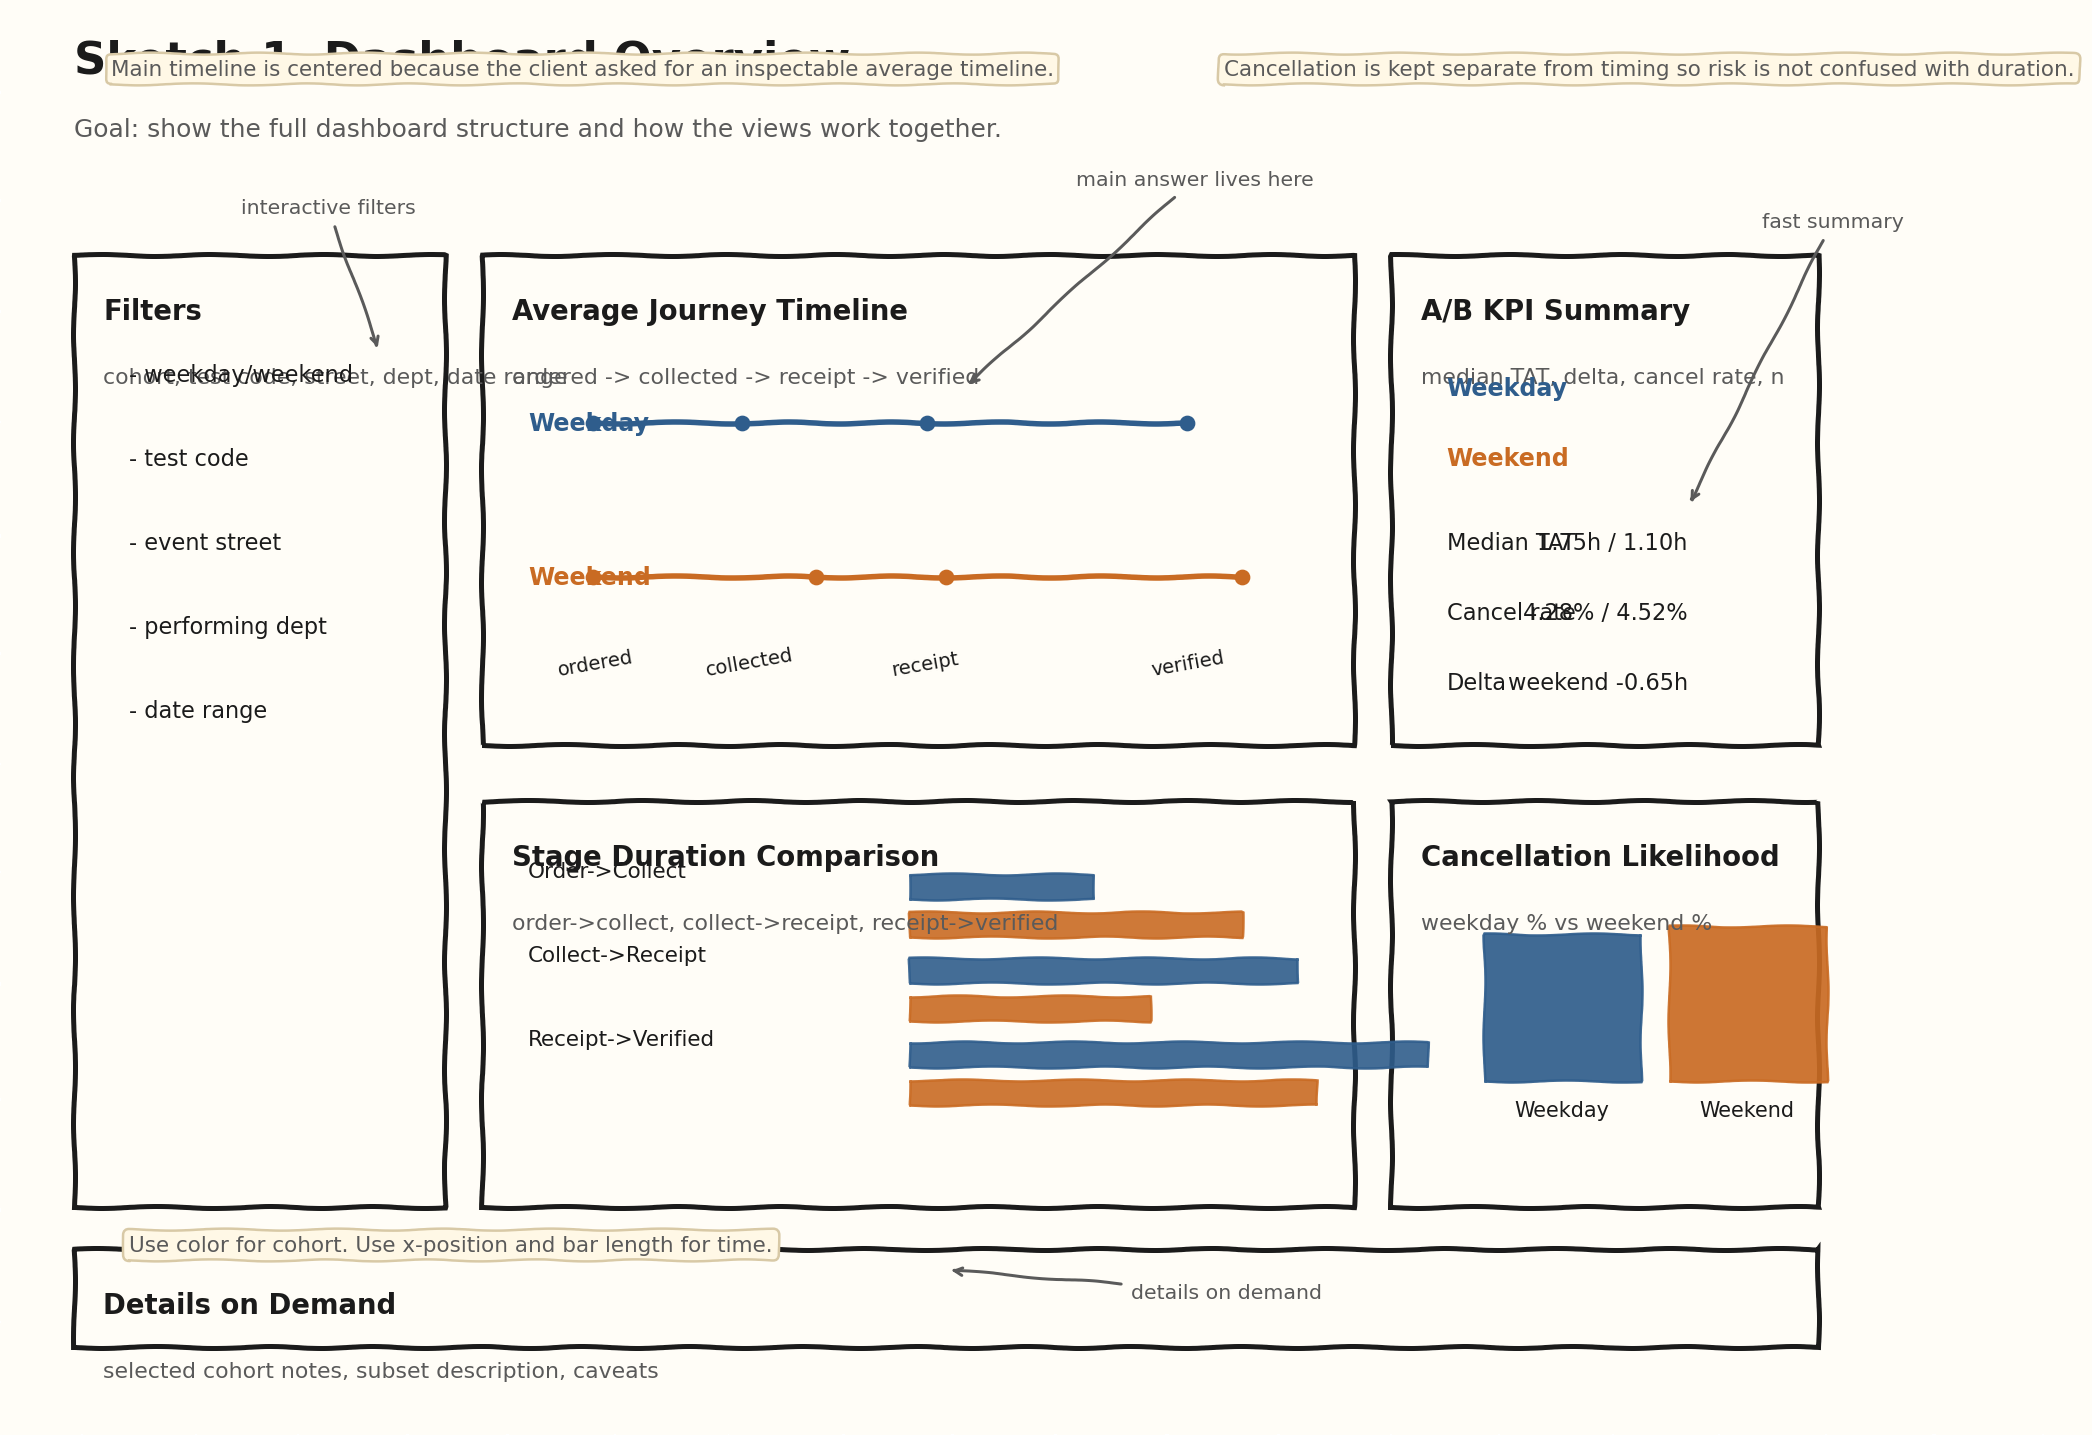
\includegraphics[width=\linewidth]{output/sketches/sketch_1_dashboard_overview.png}
    \caption{Low-fidelity dashboard layout sketch}
\end{subfigure}
\hfill
\begin{subfigure}[t]{0.32\textwidth}
    \centering
    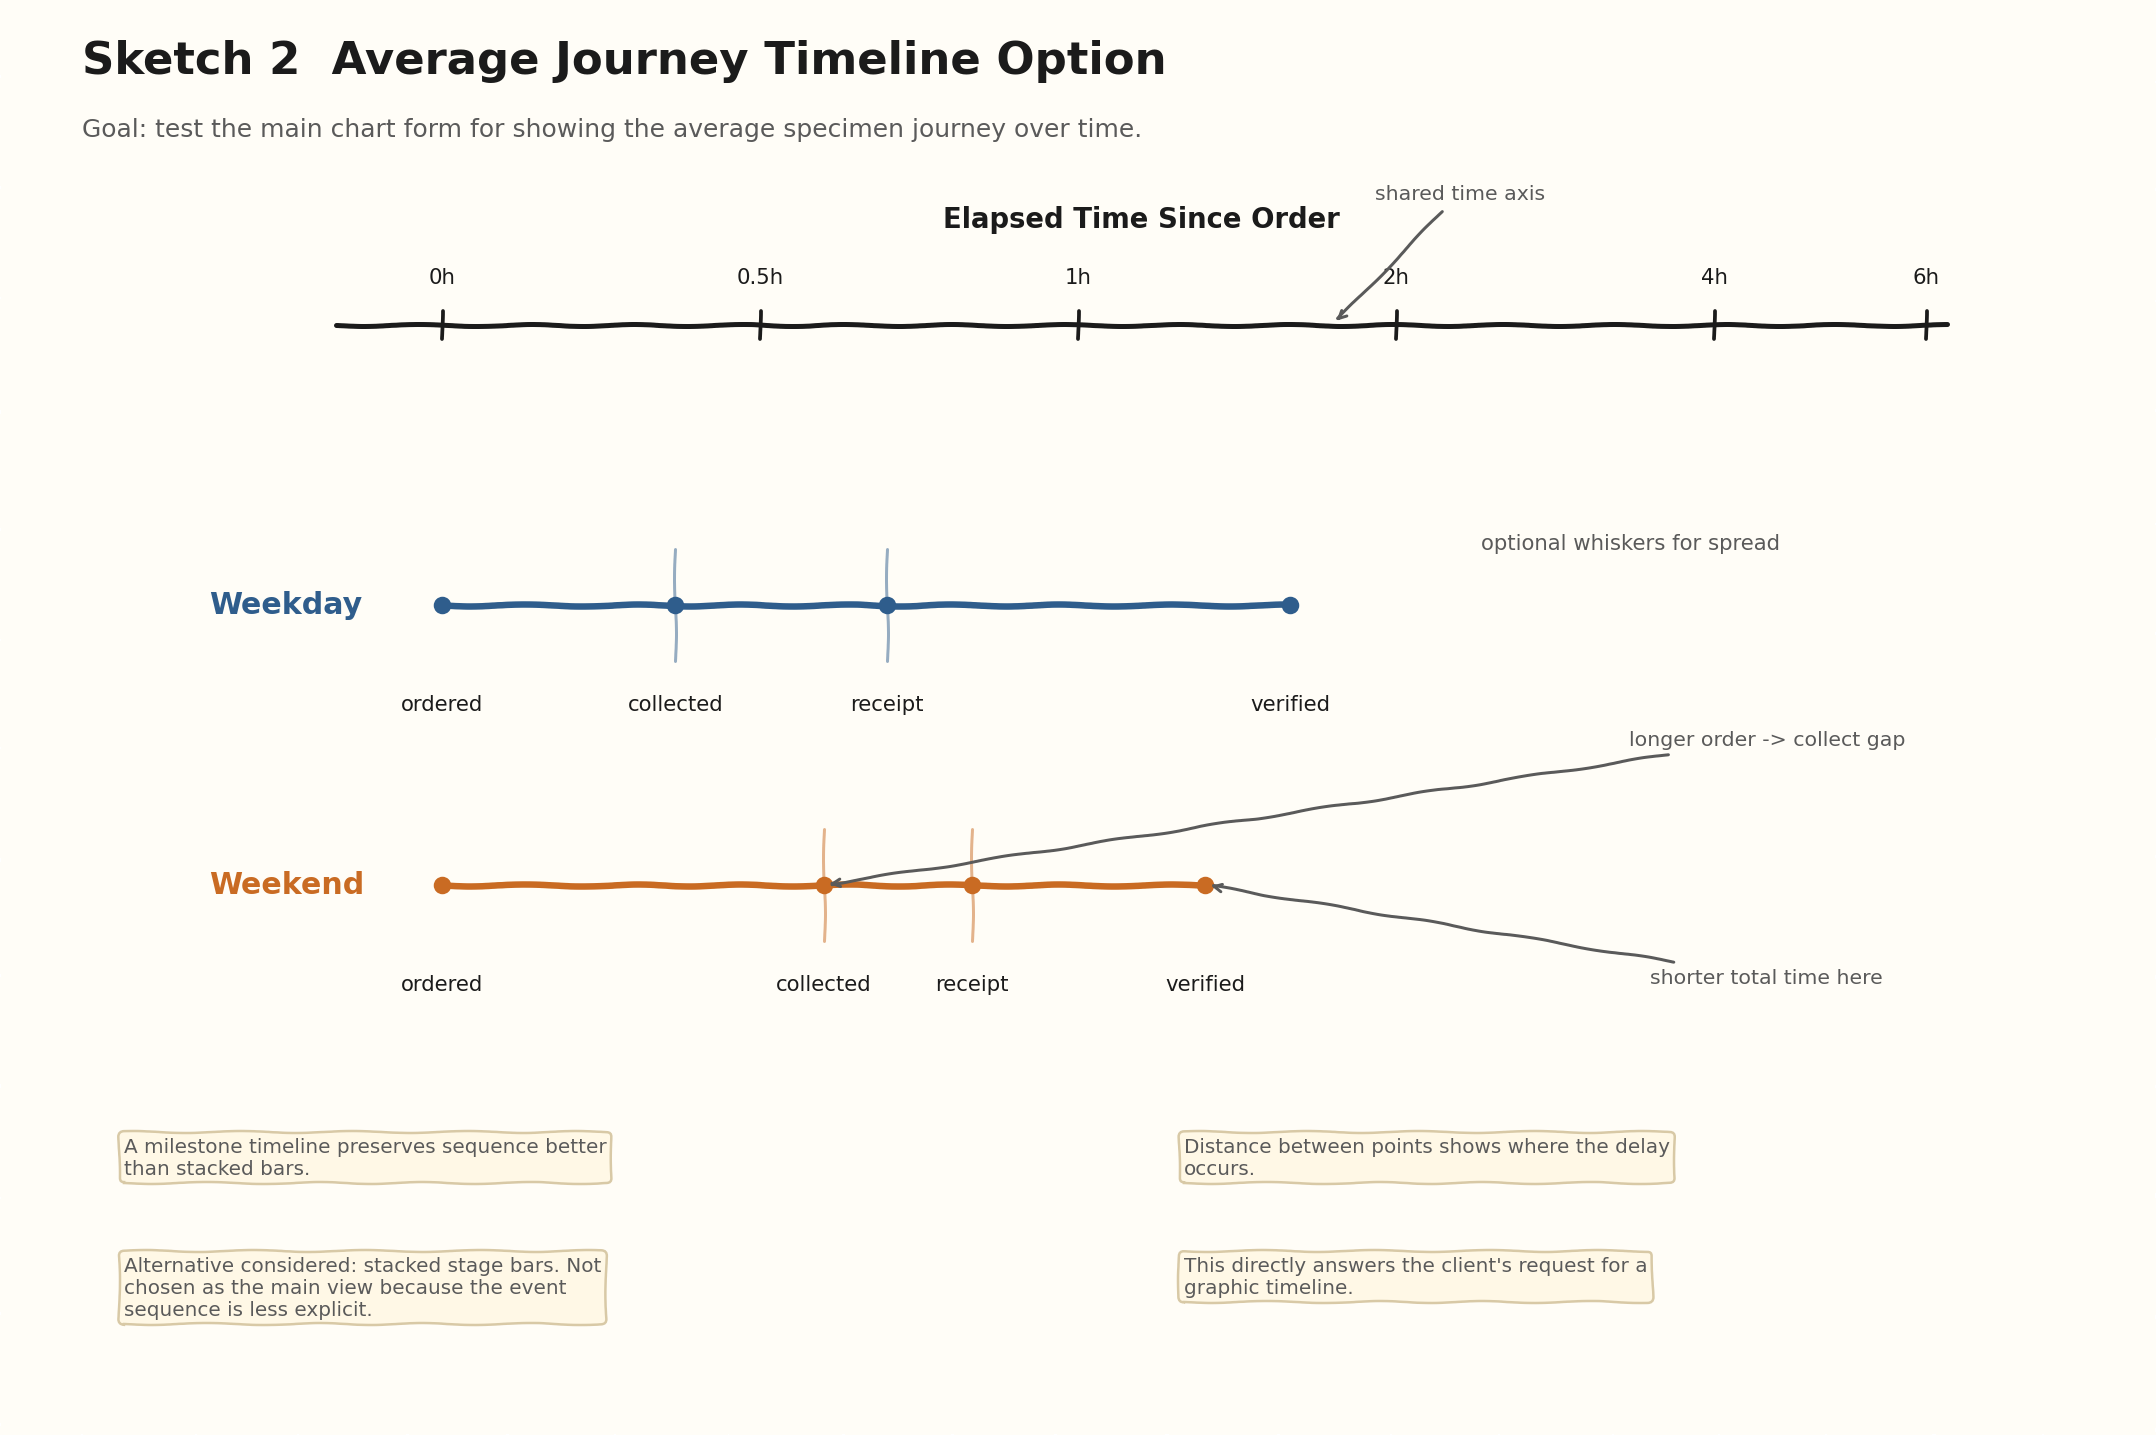
\includegraphics[width=\linewidth]{output/sketches/sketch_2_average_journey_timeline.png}
    \caption{Low-fidelity timeline sketch}
\end{subfigure}
\hfill
\begin{subfigure}[t]{0.32\textwidth}
    \centering
    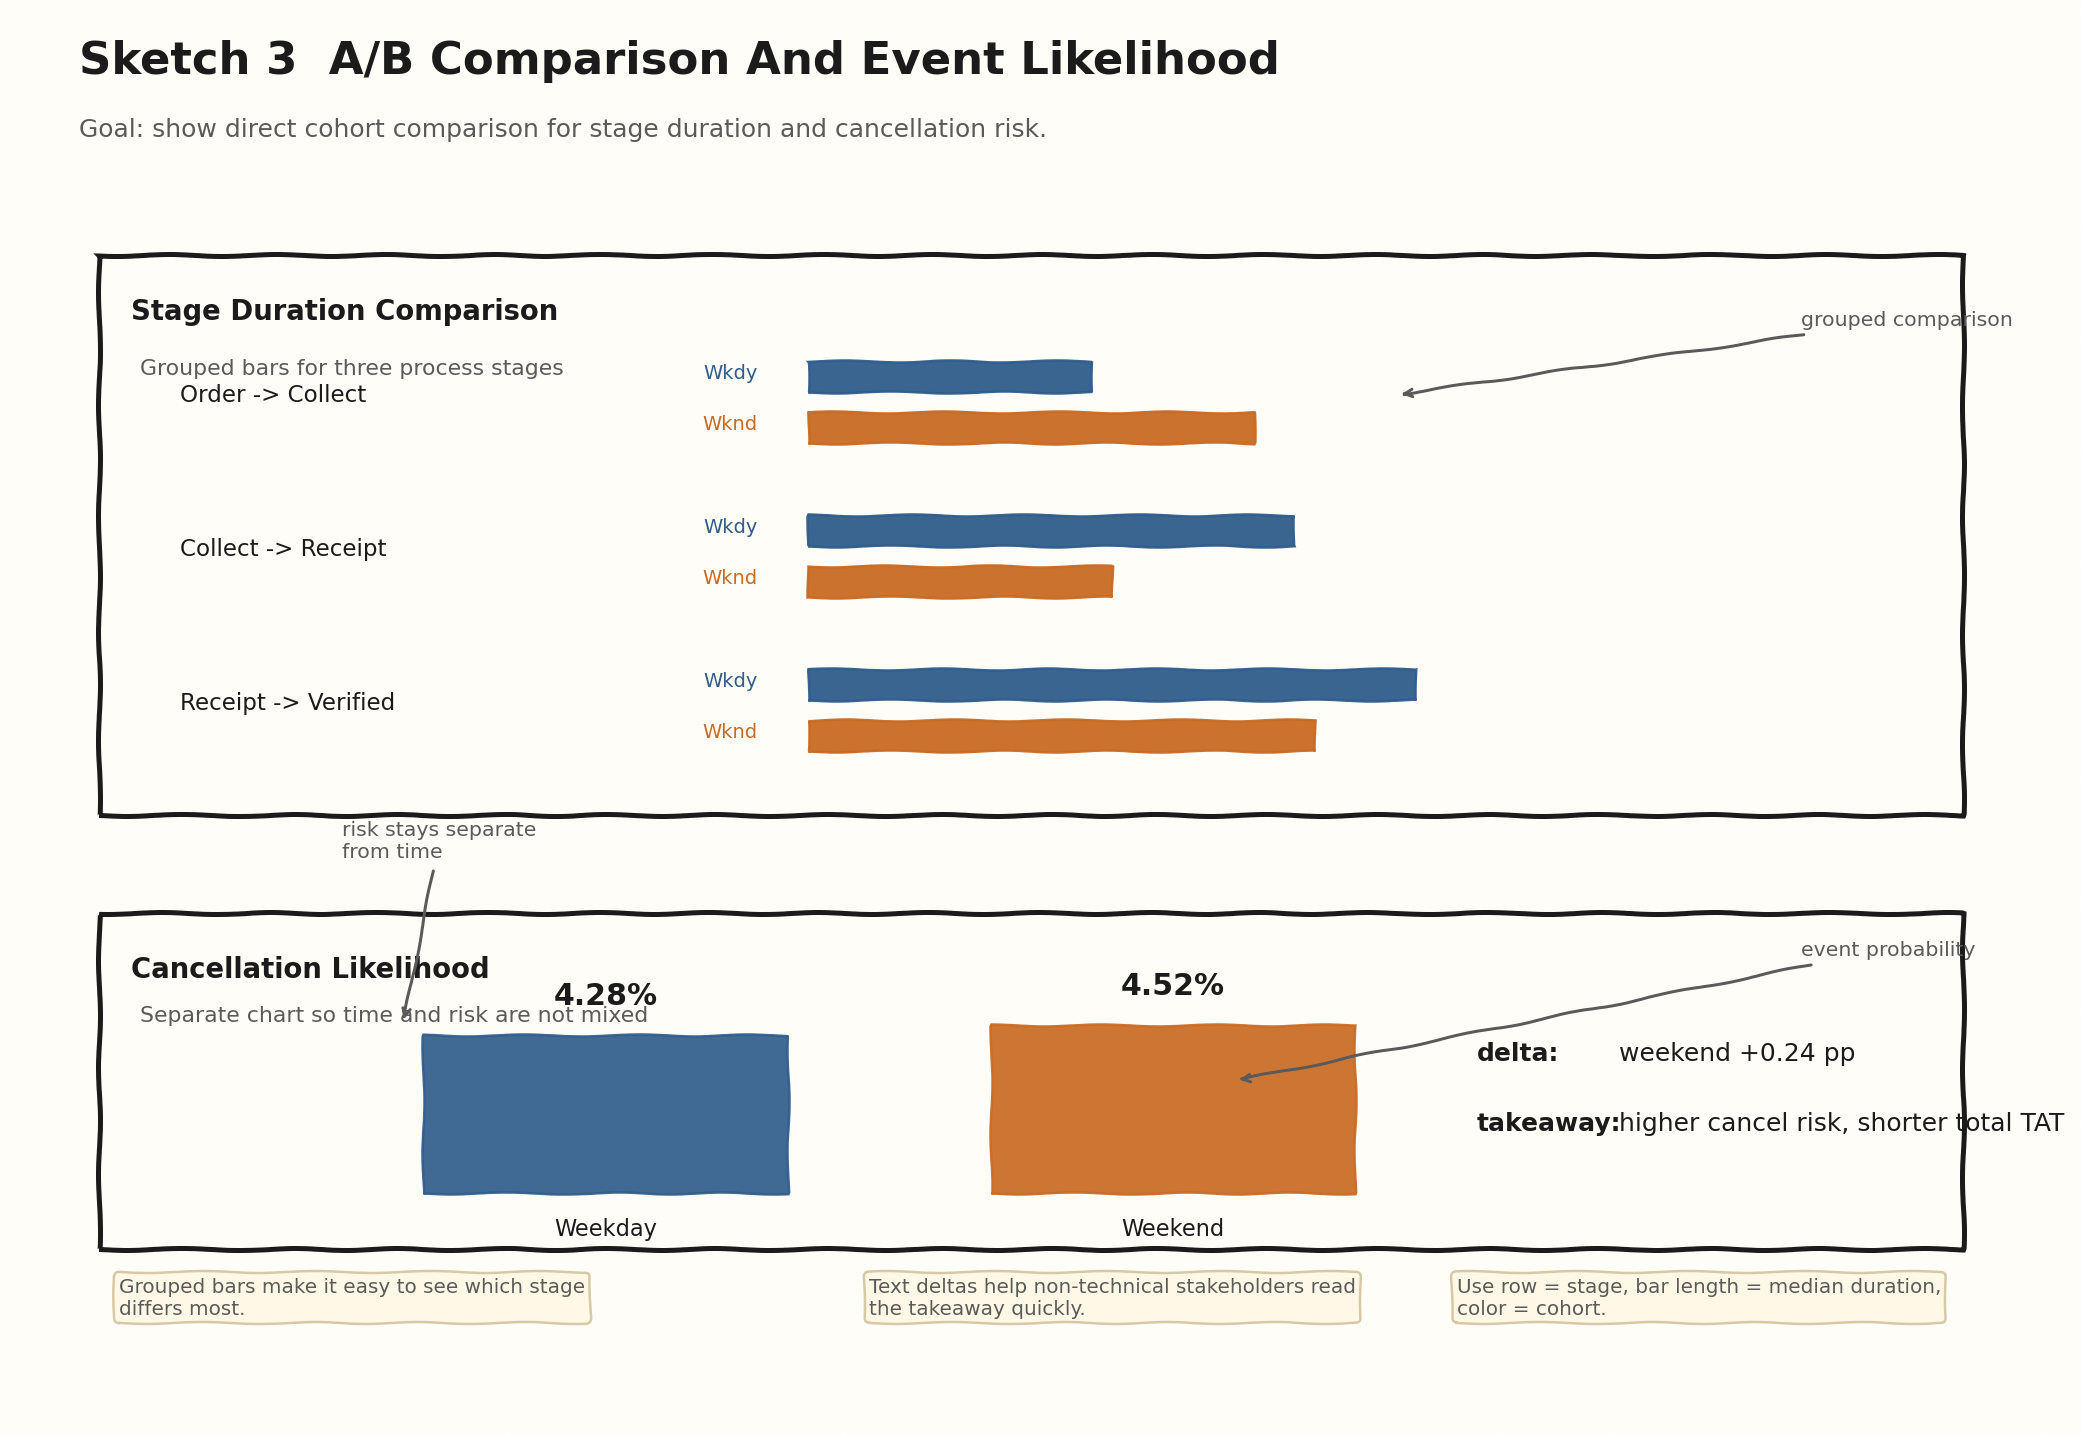
\includegraphics[width=\linewidth]{output/sketches/sketch_3_ab_comparison_and_risk.png}
    \caption{Low-fidelity A/B and risk sketch}
\end{subfigure}
\caption*{\small Figure: Early-stage digital wireframe sketches used to explore layout, encodings, and comparison views before building the final dashboard.}
\end{figure}

\end{document}
